\documentclass{article}
\usepackage[utf8]{inputenc}
\usepackage[T1]{fontenc}
\usepackage[polish]{babel}
\usepackage{geometry}
\usepackage{graphicx}
\usepackage{xcolor}
\usepackage{lmodern}
\usepackage{float}
\usepackage{pgfplots}
\usepackage{titlesec}
\usepackage{multicol}
\usepackage{listings}
\usepackage{fancyhdr}
\usepackage{tcolorbox}
\usepackage{amsmath}
\usepackage{siunitx} % dla jednostek
\usepackage{colortbl}
\definecolor{lightblue}{RGB}{204, 229, 255}
\usepackage{tikz} % dodany jawnie dla pewności
\usepackage{graphicx}  % do wstawiania obrazów
\usepackage{caption}   % (opcjonalnie) dla \caption*{}



\pgfplotsset{
	width=10cm, height=6cm, ymin=0, xmin=32, xmax=4096, grid=both,
	xticklabel style={rotate=45, anchor=near xticklabel},
	x label style={at={(axis description cs:0.5,-0.025)}},
}
% Marginesy strony
\geometry{
	a4paper,
	left=20mm,
	right=20mm,
	top=30mm,
	bottom=25mm,
	headsep=20mm,
}


% Formatowanie sekcji
\titleformat{\section}{\LARGE\bfseries\centering}{}{0em}{}

\begin{document}
	
	\lstset{
		backgroundcolor=\color{black},  % Tło czarne
		basicstyle=\ttfamily\color{white},  % Kolor tekstu biały
		keywordstyle=\color{cyan},  % Kolor słów kluczowych na niebiesko
		commentstyle=\color{gray},  % Kolor komentarzy na szaro
		stringstyle=\color{green},  % Kolor ciągów znaków na zielono
		showstringspaces=false,  % Nie pokazuj spacji w ciągach
		tabsize=3,  % Rozmiar tabulacji
		breaklines=true,  % Łamanie długich linii
		frame=none,  % Bez ramki
		xleftmargin=0cm,  % Margines po lewej stronie
		xrightmargin=0cm,  % Margines po prawej stronie
		aboveskip=0pt,  % Odstęp przed
		belowskip=0pt,  % Odstęp po
		columns=fullflexible,  % Kolumny elastyczne
		linewidth=\linewidth  % Szerokość linii na pełną szerokość
	}
	
	% Strona tytułowa
	\thispagestyle{empty} % Brak nagłówków/stopek na pierwszej stronie
	
	\begin{center}
		
\includegraphics[width=6cm]{Image/PP-PUT-LOGO.png}
		\vspace{1cm}
		
		{\Huge\bfseries Politechnika Poznańska}
		
		\vspace{1cm}
		
		{\large Informatyka rok I semestr 2} \\[0.3cm]
		L10, Piątek 11:45 - 13:15
		
		\vspace{1.5cm}
		
		{\LARGE\bfseries Algorytmy i Struktury Danych} \\[0.3cm]
		\textbf{Prowadzący:} Dominik Piotr Witczak
		
		\vspace{2cm}
		
		% Poprawione formatowanie
		{\LARGE\bfseries Sprawozdanie nr 3} 
		
		\vspace{1cm}
		
		{\Large\bfseries Sortowanie topologiczne grafów}
		
		\vspace{3cm}
		
		\begin{flushright}
			\textbf{Autor:} \\[0.2cm]
			Dominik Fischer 164176 \\
			Oliwer Miller 163544
		\end{flushright}
		
		\vspace{1.5cm}
		Rok akademicki 2024/2025
	\end{center}
	
	
	
	\newpage
	%\subsection*{Wprowadzenie}
	\titleformat{\section}[block]{\Huge\bfseries}{\thesection}{2em}{}
	\section*{\textcolor{blue}{Wprowadzenie}}
	
	\noindent Celem niniejszego grafu jest reprezentacja grafu i jego generacji oraz przedstawiene go w trzech formach: macierz grafu, lista sąsiadów i tabela. Przedstawimy również na wykresach wyniki pomiarów czasowych akcji wykonywanych na grafach, w zależności od liczby wierzchołków. 

	\section*{\textcolor{blue}{Struktura grafu}}
	
	\begin{multicols}{2}
	\noindent Klasa \textit{Graph} zawiera odwołanie do wierzchołków, wybranej reprezentacji oraz każdą z tych reprezentacji.
	
	\begin{tcolorbox}[colback=black,colframe=gray!50!,arc=3mm,boxrule=0pt,left=0pt,right=0pt,width=\linewidth]
		\textcolor{white}{\textbf{\textsf{Terminal}}}\\
		
		\begin{lstlisting}[language=Python]
		class Graph:
			def __init__(self, nodes, representation="list"):
				self.nodes = nodes
				self.representation = representation
				self.matrix = [[0] * nodes for _ in range(nodes)]
				self.adj_list = [[] for _ in range(nodes)]
				self.table = []
		\end{lstlisting}
		
	\end{tcolorbox}
	\end{multicols}
	\subsection*{\textcolor{blue}{Generacja grafu}}
	
	
	\begin{multicols}{2}
	\noindent Funkcja \textit{generate\_acyclic\_graph()} ma za zadanie wygenerowanie losowego acyklicznego grafu skierowanego z nasyceniem \textit{saturation}, którego wartość jest wprowadzana przy uruchamianiu programu z \verb|--generate|. Tworzona jest lista możliwych krawędzi idących z wierzchołka mniejszego do większego, aby uniknąć tworzenia cyklów. Następnie, na podstawie podanego nasycenia, jest wyliczana ilość krawędzi do dodania, które są losowo wybierane z listy i dodawane do grafu.
	
	\begin{tcolorbox}[colback=black,colframe=gray!50!,arc=3mm,boxrule=0pt,left=0pt,right=0pt,width=\linewidth]
		\textcolor{white}{\textbf{\textsf{Terminal}}}\\
	\begin{lstlisting}[language=Python]
		def generate_acyclic_graph(self, saturation):
			possible_edges = [(i, j) for i in range(1, self.nodes) for j in range(i + 1, self.nodes + 1)]
			max_edges = len(possible_edges)
			num_edges_to_add = round((saturation / 100) * max_edges)
			
			selected_edges = random.sample(possible_edges, num_edges_to_add)
			
			for u, v in selected_edges:
			self.add_edge(u, v)
	\end{lstlisting}
	
	\end{tcolorbox}
	\end{multicols}
	
	\section*{\textcolor{blue}{Porównanie czasów wykonania}}
	
	\begin{figure}[H]
		\centering
		\noindent\resizebox{\textwidth}{!}{
			\begin{tikzpicture}
				\begin{axis}[%
					name=plotA, anchor=left of south west,
					width=10cm, height=4cm,
					title={Złożoność Obliczeniowa - Find}, 
					xlabel={Rozmiar instancji}, ylabel={Czas (ms)}, legend pos=north west,
					xmode=log, log basis x={2},
					every axis plot post/.style={very thick},
					]
					\addplot[red, dashed, smooth] table[x=nodes,y=time,col sep=comma] {results/find_matrix.csv};
					\addplot[green, dashed, smooth] table[x=nodes,y=time,col sep=comma] {results/find_table.csv};
					\addplot[blue, dotted, smooth] table[x=nodes,y=time,col sep=comma] {results/find_list.csv};
					\legend{Matrix, Table, List}
				\end{axis}
				
				\begin{axis}[%
					title={Złożoność Obliczeniowa - Kahn}, 
					width=10cm, height=4cm,
					name=plotB, at=(plotA.below south west), anchor=above north west,
					xlabel={Rozmiar instancji}, ylabel={Czas (ms)}, legend pos=north west,
					xmode=log, log basis x={2},
					every axis plot post/.style={very thick},
					]
					\addplot[red, dashed, smooth] table[x=nodes,y=time,col sep=comma] {results/kahn_matrix.csv};
					\addplot[green, dashed, smooth] table[x=nodes,y=time,col sep=comma] {results/kahn_table.csv};
					\addplot[blue, dotted, smooth] table[x=nodes,y=time,col sep=comma] {results/kahn_list.csv};
					\legend{Matrix, Table, List}
				\end{axis}
				
				\begin{axis}[%
					title={Złożoność Obliczeniowa - Tarjan}, 
					width=10cm, height=4cm,
					name=plotC, at=(plotB.below south west), anchor=above north west,
					xlabel={Rozmiar instancji}, ylabel={Czas (ms)}, legend pos=north west,
					xmode=log, log basis x={2},
					every axis plot post/.style={very thick},
					]
					\addplot[red, dashed, smooth] table[x=nodes,y=time,col sep=comma] {results/tarjan_matrix.csv};
					\addplot[green, dashed, smooth] table[x=nodes,y=time,col sep=comma] {results/tarjan_table.csv};
					\addplot[blue, dotted, smooth] table[x=nodes,y=time,col sep=comma] {results/tarjan_list.csv};
					\legend{Matrix, Table, List}
				\end{axis}
			\end{tikzpicture}
		}
		\caption{Porównanie czasów wykonania dla 3 operacji i 3 reprezentacji grafów}
	\end{figure}
	
	\section*{\textcolor{blue}{Generowanie i wypisanie grafu}
	\begin{figure}[htbp]
		\centering
		\begin{minipage}[b]{0.3\textwidth}
			\centering
			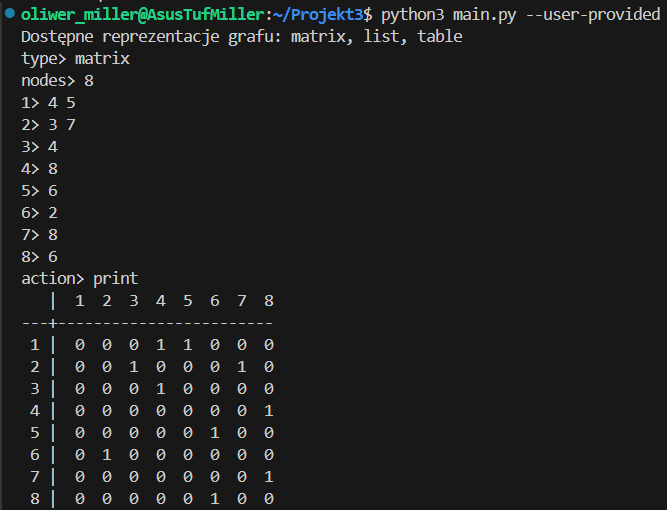
\includegraphics[width=\textwidth]{reprezentacja_matrix.png}
			\par\small (a) Macierz grafu
		\end{minipage}
		\hfill
		\begin{minipage}[b]{0.3\textwidth}
			\centering
			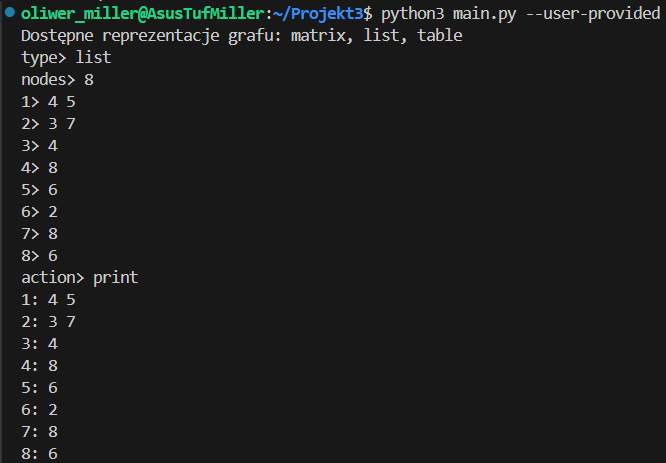
\includegraphics[width=\textwidth]{reprezentacja_list.png}
			\par\small (b) Lista
		\end{minipage}
		\hfill
		\begin{minipage}[b]{0.3\textwidth}
			\centering
			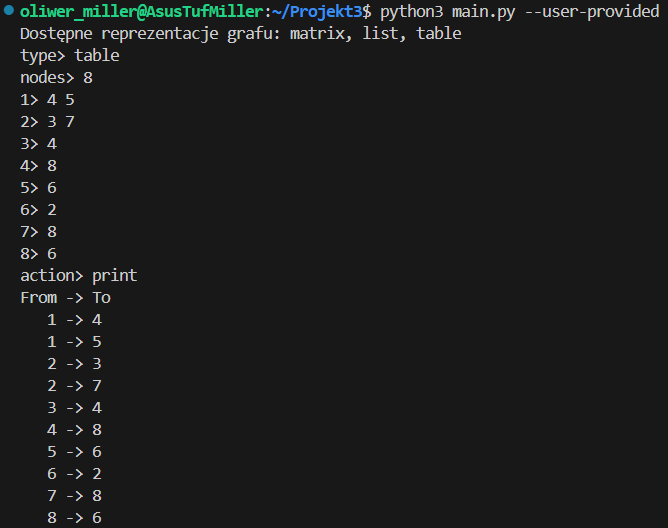
\includegraphics[width=\textwidth]{reprezentacja_table.png}
			\par\small (c) Tabela
		\end{minipage}
		\caption{Trzy obrazki obok siebie}
		\label{fig:trzy-obrazki}
	\end{figure}
	
	
	
	%\subsection*{Podsumowanie}
	\section*{\textcolor{blue}{Wnioski}}
	\noindent Akcja Find ma za zadanie sprawdzić czy istnieje krawędź między dwoma danymi wierzchołkami. Wszystkie reprezentacje grafu wypadają tak samo dobrze do wielkości danych około $2^{10}$. Przy większych danych złożoność obliczeniowa Find w macierzy grafu znacznie wzrasta. W przypadku listy złożoność też wzrasta, jednak nie tak gwałtownie, a dla tablicy złożoność pozostaje taka sama.
	\\ W sortowaniu topologicznym algorytmem Kahna wszystkie reprezentacje wypadają bardzo podobnie, jedynie w dla danych o wielkości około $2^{11}$ dana akcja wykonuje się szybciej dla macierzy grafu.
	\\ W sortowaniu topologicznym algorytmem Tarjana złożoność obliczeniowa dla tablicy wzrasta od rozmiaru danych wynoszącemu $2^{10}$ elementów. Złożoność obliczeniowa dla macierzy i listy pozostaje stała.
	
\end{document}
